\section{Tabela de Decisão}\label{sec:tab_dec}
A tabela de decisão contém a memória das últimas
decisões $a_{old} \in A_c$ de todos os robôs de $T_c$.
Isso é incorporado ná próxima rodada do algorítmo,
conforme ilustrado na figura~\ref{fig:tab_dec}.

\begin{figure}
  \centering
  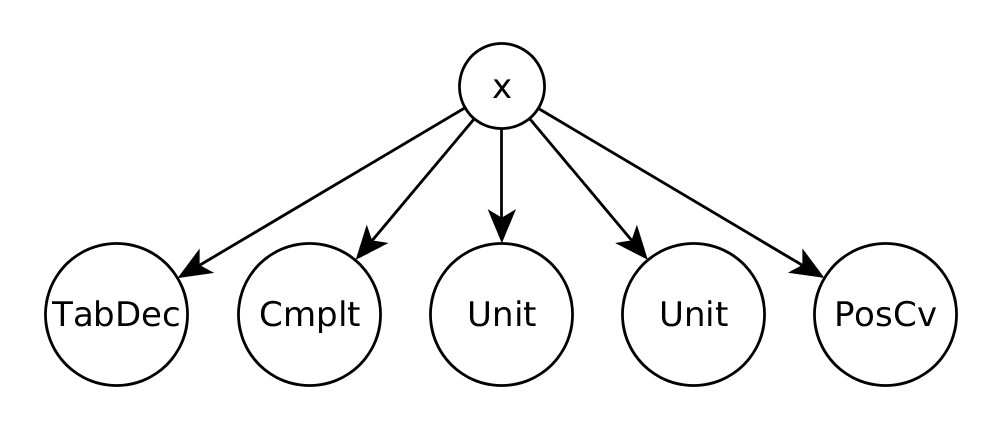
\includegraphics[width= 0.8\linewidth]{tab_dec}
  \caption{Ilustração da distribuiçao dos tabuleiros
           considerados no planejamento}\label{fig:tab_dec}
\end{figure}

Os tipos de ações que são geradas são:
\begin{itemize}
  \item \textit{TabDec}: Ação escolhida no último planejamento
  \item \textit{Unit}: Ação gerada a partir da tabela de decisão
        onde a ação de um único robô foi modificada
  \item \textit{Cmplt}: Ação gerada a partir da tabela de decisão
        onde a ação do time completo foi modificada
  \item \textit{PosCv}: Ação gerada utilizando posições chave
        (vide secção~\ref{sec:pos_chave})
\end{itemize}

Devido a movimentação dos robôs em $Rob_{ad}$, somente as
ações $Mover(r_i)$ e $Chutar(r_{com{\ }bola})$ são guardadas
intergralmente. No caso da ação $Passar(r_j, r_{com{\ }bola})$,
devido a restrição de o robô que recebe interceptar a bola
antes dos robôs em $Rob_{ad}$, o calculo do receptor $r_j$ é
feito a cada rodada. O receptor anterior só entra no custo
da mudança (vide secção~\ref{subsec:change_cost}). 

Caso a posse de pola passe para o time adversário, o robô
que possuia a bola anteriormente fica com a sua última
ação do tipo $Mover(r_i)$.
